\section{Введение}

Точность измерения параметров элементарной ячейки (ПЭЯ) монокристаллов на дифрактометрах, оборудованных 2D-детекторами, обсуждается достаточно активно~\cite{Herbstein:2000,Waterman:2010,Dudka:2010,Henn:2019,Taylor:1986,Serebrennikova:2021}.
В работе~\cite{Dudka:2017} проблема сформулирована следующим образом: <<\ldotsпопытки получить воспроизводимые значения параметров элементарных ячеек монокристаллов при повторных исследованиях или исследовать зависимости этих параметров от температуры или давления могут привести к разочарованию>>.
К этому можно добавить, что это утверждение справедливо и при сопоставлении данных рентгеноструктурного анализа (РСтА) монокристаллов и дифрактометрии поликристаллов.
Трудно перечислить все подходы, предложенные для минимизации ошибок измерения ПЭЯ монокристаллов.
Среди последних обзоров на эту тему можно указать~\cite{Galdecka:2006,Lider:2020}.
Возможности методик с использованием внешнего или внутреннего эталонов на ряде примеров продемонстрированы в работах~\cite{Gromilov:2022,Panchenko:2022,Panchenko:2023,Serebrennikova:2023,Serebrennikova:2022}.
Особо следует отметить, что эти методики ориентированы на исследование малых монокристаллов (т.е. имеющих размер меньше первичного пучка), пригодных для проведения РСтА.
Пробоотбор подходящих для исследования образцов такой же, как и для РСтА --- требуется совершенный кристаллик с линейными размерами <0.1~мм.
Дополнительное требование --- наличие рефлексов с разрешенным дублетом, если оно выполняется, то при использовании рефлексов с $2\theta \approx 120\degree$ и гониометров с точностью $0.005\degree$ можно рассчитывать на измерение межплоскостных расстояний с относительной ошибкой не хуже $\Delta d / d = 5 \cdot 10^{-5}$.
Не во всех случаях использование внутреннего эталона удобно, т.к. требует дополнительных усилий при подготовке и определении ориентации одновременно обоих кристаллов, а также приводит к уменьшению интенсивности и взаимному экранированию~\cite{Serebrennikova:2022}.
Использование внешнего эталона обычно вызывает вопросы об эквивалентности установки образцов.
В этом плане развитие безэталонных методик имеет свои перспективы.

Классической безэталонной методикой измерения ПЭЯ является схема Бонда~\cite{Bond:1960}, в основе которой лежат два основных фактора – наличие точного гониометра (достаточно одноосного) и сориентированной определенным образом монокристаллической пластинки (см. рис.~\ref{fig:bond}а).
Методика хорошо себя проявила на малых кристаллах~\cite{Lisoivan:1988}, хотя при использовании одноосных гониометров в случае кристаллов средних и низших сингоний требуется переклейка кристалла.
Современные монокристальные дифрактометры оснащаются моторизированными гониометрами позволяющими поворачивать образец вокруг двух- или трех осей, что делает их подходящими для реализации схемы Бонда.
Причем эту схему можно реализовать как на больших ориентированных монокристаллических пластинах, так и на малых кристаллах.
Если при измерениях на больших кристаллах (см. рис.~\ref{fig:bond}а) угол $2\theta = \omega_+ - \omega_-$ свободен от ошибок, связанных со смещением образца с оси гониометра, то во втором необходимо учитывать возможное смещение, т.е. эксцентриситет.
Эксцентриситет зависит как от размера сферы сведения осей (\textit{sphere of confusion}), так и точности центрирования образца.
Подходы к экспериментальному учету эксцентриситета малых монокристаллов достаточно хорошо проработаны в литературе см., например,~\cite{Ponomarev:1969,King:1979}.

\begin{figure}[ht!]
    \centering
    \begin{subfigure}{0.5\textwidth}
    \centering
    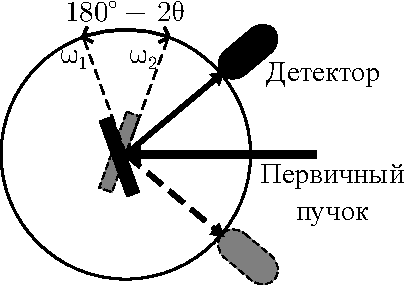
\includegraphics[]{bond.pdf}
    \caption{}%
    \label{fig:bond}
    \end{subfigure}%
    \begin{subfigure}{0.5\textwidth}
    \centering
    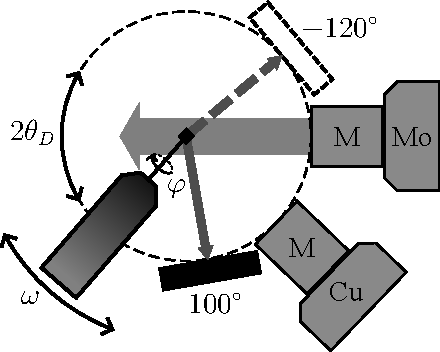
\includegraphics[]{our_bond.pdf}
    \caption{}%
    \label{fig:our_bond}
    \end{subfigure}
    \caption{Схемы эксперимента для учета эксцентриситета образца.}%
\end{figure}

Кроме этого, точность измерения ПЭЯ зависит от точности гониометра.
В паспорте сейчас обычно указывают лишь воспроизводимость установки углов, и не указывают значение самой погрешности.
Другие ошибки, возникающие при использовании серийных приборов, ориентированных на проведение РСтА, обусловлены значительной расходимостью первичного пучка (на уровне нескольких десятых градуса).
На точность измерений влияет и общая компоновка гониометра: при горизонтальном расположении рентгеновской трубки доступные для съемки углы $2\theta$ значительно ограничены.
Использование 2D-детектора также ограничивает углы $2\theta$, а также предполагает обработку двумерных профилей, что вносит свои нюансы в определение положения максимума, особенно при неполном разрешении дублета.
В основе точности измерений ПЭЯ в схеме Бонда лежит значение использованной длины волны, далее будут использованы рекомендованные значения $\lambda \text{Mo} K \alpha_1 = 0.70931715 (41)\unit{\AA}$ и $\lambda \text{Mo} K \alpha_2 = 0.713607 (12)\unit{\AA}$~\cite{Deslattes:1985}.

Проведение измерений ПЭЯ с максимально достижимой точностью всегда было особым разделом рентгенографии.
Уже для первых дифрактометров был предложен ряд подходов к учету основных приборных ошибок~\cite{Ponomarev:1969}. В~\cite{King:1979} предложен метод учета основных ошибок по результатам съемки 8 рефлексов на приборе, оснащенном четырехкружным гониометром и точечным детектором.
Цель настоящей работы --- оценка и учет ошибок измерений ПЭЯ, связанных с эксцентриситетом образца, в схеме Бонда на современных дифрактометрах.
Для этого логично привлечь эталонные образцы, для которых ПЭЯ известны с хорошей точностью.
